\graphicspath{ {Figures/VW/} }

\chapter{Analysis Procedures}
\label{Ch:Procedures}


\section{Key parameters in reconstruction method}

	Default parameters used in the Recon West production of the 60H dataset, with SAM dataset name ``gm2pro\_daq\_full\_run1\_60h\_5033A\_withfullDQC''.

\section{Analysis Data Preparation Procedure}

	\begin{itemize}
		\item{git branch: gm2analyses branch feature/KinnairdAnalyses}
		\item{Majority of code located under gm2analyses/macros/RatioMacro}
	\end{itemize}

	\begin{enumerate}
		\item{Submit jobs to OSG to run the rootTreesAndLostMuons.fcl file which produces root trees of positron hits using the ClusterTree analyzer module and coincident MIP hits using the TestCoincidenceFinder analyzer module.}
		\item{Submit jobs to Fermigrid to produce histograms from root trees using the ClusterTreeToHistsPileup.C macro in RatioMacro/HistMaking. Beyond standard threshold histograms this macro produces pileup and lost muon histograms all within the same root file.}
	\end{enumerate}


\section{Histogramming Procedure}

	Method: Weighted Ratio (threshold)

	\begin{enumerate}
		\item{Loop through all clusters and apply an artificial deadtime (ADT) to combine hits within 6 ns into a single pulse using the same procedure and code that the pileup method uses (see below). Drop clusters with time $< \SI{25}{\mu s}$ or time $> \SI{600}{\mu s}$.}
		\item{Histograms are constructed with ROOT's TH1F class with 149.15 ns bins from $0 - \SI{699.96095}{\mu s}$ corresponding to 4693 bins.}
		\item{Randomize times by $\pm 149.15/2$ ns and fill histograms for energies $> 1.7$ GeV. Randomization uses ROOT's default TRandom3 class.}
		\item{Fill one of the four histograms \{$u_{+}(t), u_{-}(t), v_{1}(t), v_{2}(t)$\} as shown in Equation \ref{eqn:fourHists} per cluster. The associated histogram is determined by generating a random number between 0 and 1, and comparing that number to the relative probabilities of the different weights.}
		\item{Clusters filled into the $u_{+}(t)$ histogram have their times shifted by $t \rightarrow t - T_{a}/2$ and clusters filled into the $u_{-}(t)$ histogram have their times shifted by $t \rightarrow t + T_{a}/2$.}
		\item{$T_{a}$ is known a priori to high precision from the previous experiment, and its value is taken as $1/f_{a}$, where $f_{a}$ is \SI{0.2291}{MHz}:
			\begin{align}
				T_{a} \approx \SI{4.364906}{\mu s}
			\label{eq:Ta}
			\end{align}}
	\end{enumerate}


\section{Gain Correction Procedure}

	Gain correction method: Default by the Italian Calibration Team

	\begin{enumerate}
		\item{Long term gain is corrected using out-of-fill lasers included normalization from the Source Monitor.}
		\item{In-fill gain is corrected using in-fill lasers including normalization from the Source Monitor.}
		\item{Short-term double pulse (SDTP) effect is not included.}
	\end{enumerate}


\section{Pileup Correction Procedure}
\label{Sec:PileupCorrection}

	Pileup correction method: Asymmetric shadow window

	\begin{enumerate}
		\item{Create a vector of clusters per calorimeter per fill. For each cluster look for a second cluster in a window from 12-18 ns after the time of the first cluster. This corresponds to a shadow dead time (SDT) of 6 ns and a shadow gap time (SGT) of 12 ns, equal to 1 and 2 times the applied ADT respectively.}
		\item{Create shadow doublets with energies and times as:
			\begin{gather}
				E_{doublet} = C \cdot (E_{1} + E_{2}), \\
				t_{doublet} = \frac{t_{1} \cdot E_{1} + (t_{2}-SGT) \cdot E_{2}}{E_{1} + E_{2}},
			\end{gather}
		where the latter equation is just the energy-weighted time between the two singlets. In the former equation, the calculation of the doublet energy is the sum of the singlets times some factor. That factor is set equal to 1, which is a decent approximation since the spatial separation in the reconstruction is turned off, and because the Short Term Double Pulse (SDTP) improvement to the laser energy calibration will be applied. The systematic effects of a factor not equal to 1 are studied in Section \ref{SubSec:PileupPhase}.}
		\item{Randomize $t_{doublet}$ times by $\pm 149.15/2$ ns as in the histogramming procedure described above.}
		\item{For each calorimeter construct a pileup spectrum P = doublets - singlets = D - S, where the singlets are subtracted at time $t_{doublet}$ as opposed to their individual times, and pulses are only added or subtracted if they are above 1.7 GeV. Subtract P off energy and threshold histograms.}
		\item{For pileup subraction in the ratio method, randomly split associated doublets and singlets into 4 separate histograms as is done in the histogramming procedure described above, with times shifted accordingly. Subtract 4 pileup histograms off corresponding \{$u_{+}(t), u_{-}(t), v_{1}(t), v_{2}(t)$\} histograms before forming the ratio.}
		\item{The errors of the pileup corrected histogram were determined to be: 
			\begin{gather}
				\sigma(N_{corrected}) = \sqrt{N_{corrected} + 2 N_{1} + 6 N_{4}},
			\end{gather}
		where $N_{1}$ is the number of doublets where both singlets were below threshold, and $N_{4}$ is the number of doublets where both singlets were above threshold, and this is a quantity evaluated at each time bin. (Cite this? DocDB 14830. Derive this in the appendix?) A histogram of error multipliers was created by factoring out the $N_{corrected}$ term, which is then applied to the bin errors before fitting. This is true even for the ratio errors to good approximation. (Cite this? Derive it as JP did?) Note that I did not time randomize the $N_{1}$ and $N_{4}$ entries when constructing the correct errors, which should have a negligble effect.}
		\item{The pileup correction at the triplet/contamination level is not included. The machinery exists to apply such a correction, but it requires more work to get it correct. It has been determined not be necessary for the 60H and Run 1 data.}
	\end{enumerate}


\section{Lost muon spectrum extraction procedure}

	Method: Triple coincidence of clusters

	Note that the lost muons are not included in the ratio fit because the ratio method divides out such slow effects. This is reflected by the lack of a low frequency peak in the FFT of the fit residuals for the ratio fit, whereas such a peak exists for T method fits. I include here however my method for extracting the lost muon function for possible future systematic studies.

	\begin{enumerate}
		\item{Triple coincidence of clusters in 3 consecutive calorimeters are made with an energy cut of 100 MeV $<$ E $<$ 250 MeV and 5 ns $<$ dt $<$ 8.5 ns.}
		\item{A time histogram is made with the muon cluster in the first calorimeter.}
		\item{The function that would be used in the final fit is:
			\begin{gather}
				\Lambda(t) = 1 - \kappa_{loss} \int_{0}^{t} L(t')e^{(-t'/\gamma\tau_{\mu})} dt'
			\end{gather}
		where $L(t)$ is the triples histogram, and an arbitrary $10^{-6}$ factor has been absorbed into $\kappa_{loss}$ in order to bring it to a more reasonable value (from $\mathcal{O}(10^{-10})$ to $\mathcal{O}(10^{-4})$).}
	\end{enumerate}


\section{Beam Dynamics: CBO Model}
\label{Sec:CBO}

	\begin{enumerate}
		\item{The CBO frequency as a function of time is taken from the tracking analysis, DocDB 14208. The CBO frequency is not constant because the quad voltage was not constant as a function of time. As described in that DocDB, the source of this is almost certainly the fact that some of the quad resistors were damaged, leading to longer RC time constants. The form used is 
			\begin{gather}
				\omega_{cbo}(t) = \omega_{0}(1 + \Delta\omega t + A e^{-t/\tau_{A}} + B e^{-t/\tau_{B}})
			\end{gather}
		with parameters determined from station 12 in the 60H dataset and fixed in the fit as:
			\begin{equation*}	
			\begin{aligned}
			 	\Delta\omega &= \SI{1.86e-8}{ns^{-1}}, \\
			 	A &= -0.0504, \\
			 	\tau_{A} &= \SI{73.3}{\mu s}, \\
			 	B &= -0.131, \\
			 	\tau_{B} &= \SI{16.6}{\mu s}. \\
			\end{aligned}
			\end{equation*}
		The parameter $\omega_{0}$ is allowed to float in the fit and starts with a value of $\SI{2.3051}{rad.\mu s^{-1}}$. The ratio method has trouble with letting the other parameters float, and fixing them to various values does not change the fit results significantly.}
		\item{Because the ratio method divides out the CBO partially (reduction by a factor of $\sim5$ in the FFT cbo peak amplitude), the ratio fit has a hard time fitting the CBO lifetime. Therefore $\tau_{cbo}$ is fixed to $\SI{180}{\mu s}$, determined from a T Method fit to the same data.}
		\item{An exponential function is assumed for the CBO decoherence.}
		\item{The $N_{cbo}$ term is included in the fit, $A_{cbo}$ and $\phi_{cbo}$ are excluded. The 2CBO term is excluded.}
		\item{The final CBO function is:
			\begin{gather}
					N_{cbo}(t) = C(t) = 1 + A_{cbo} e^{-t/\tau_{cbo}} \cos(\omega_{cbo}(t)t + \phi_{cbo})
			\label{eqn:CBO}
			\end{gather}
		}
	\end{enumerate}


\section{Beam Dynamics: Vertical Waist Model}
\label{Sec:VW}

	\begin{enumerate}
		\item{\wa is senstive to the width of the beam, which is characterized by the frequency 
			\begin{gather}
				f_{VW} = f_{cyc} - 2f_{y}, \\
				f_{y} = f_{cbo} \sqrt{\frac{2f_{cyc}}{f_{cbo}} - 1}.
			\end{gather}}
		\item{An exponential function is assumed for the VW decoherence as in the CBO, and so the VW term is defined as
			\begin{gather}
					V(t) = 1 + A_{VW} e^{-t/\tau_{VW}} \cos(\omega_{VW}t + \phi_{VW})
			\end{gather}
		}
		\item{$\omega_{VW}$ is assumed to be a constant value even though the CBO frequency changes vs time.}
	\end{enumerate}

	In the 60H dataset $f_{VW} \approx \SI{2.3}{MHz} \approx 10 \cdot \omega_{a}$, which is an even multiple of the \gmtwo frequency. It turns out that any frequencies which are even multiples of the \gmtwo frequency largely cancel in the ratio. This is shown for the vertical waist in Figure \ref{fig:VWPlot}. This combined with the time randomization to remove the fast rotation ($f_{cyc}$) means the vertical waist does not need to be included in the ratio fit. This is justified by the lack of a vertical waist peak in the FFT of the residuals of the fit, as will be shown later.

	\begin{figure}[]
		\centering
		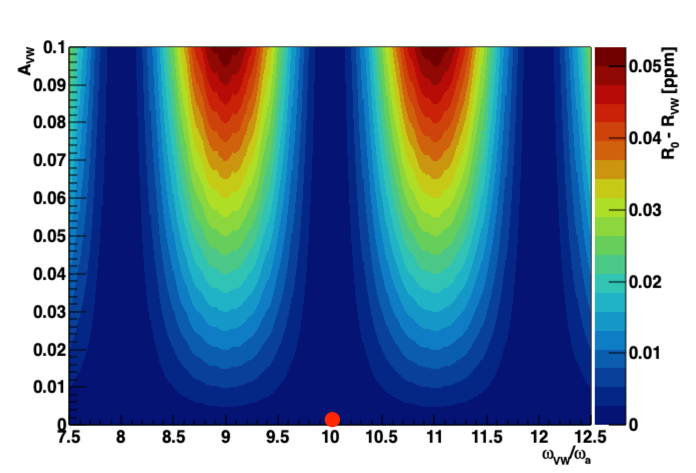
\includegraphics[width=\textwidth]{VWPlot}
	    \caption[VWPlot]{Plotted is the difference in the maximum value of the ratio with a vertical waist function included and without, as a function of both the amplitude of the vertical waist effect and the vertical waist frequency in units of the \gmtwo frequency. This was created with a toy Monte Carlo. As is shown the difference reaches a minimum for even multiples of the \gmtwo frequency. The 60H dataset lives at the bottom center of this plot, where the difference in the ratio is approximately \SI{5e-6}{} at 30 $\mu s$. Plot created by James Mott.}
	    \label{fig:VWPlot}
	\end{figure}


\section{Final Fit Function}
\label{Sec:FinalFitFunction}

	The following function is used for the final fit for each calorimeter and for the calorimeter sum:
	\begin{gather}
			R(t) = \frac{2f(t) - f_{+}(t) - f_{-}(t)}{2f(t) + f_{+}(t) + f_{-}(t)} \\[10pt]
			f_{\pm}(t) = f(t \pm T_{a}/2) \\[10pt]
			f(t) = C(t) (1 + A \cos(\omega_{a}t + \phi)) \\[10pt]
			C(t) = 1 + A_{cbo} e^{-t/\tau_{cbo}} \cos(\omega_{cbo}(t)t + \phi_{cbo}) \\[10pt]
			\omega_{a} = 2 \pi \cdot \SI{0.2291}{MHz} \cdot (1 + R \times 10^{-6})
	\end{gather}
	All parameters are floating except for terms in $\omega_{cbo}(t)$ and $\tau_{cbo}$ as described above.



